% Chapter Template

\chapter{Introduction} % Main chapter title

\label{Chapter 1} % Change X to a consecutive number; for referencing this chapter elsewhere, use \ref{ChapterX}

\lhead{Chapter 1. \emph{Introduction}} % Change X to a consecutive number; this is for the header on each page - perhaps a shortened title

%----------------------------------------------------------------------------------------
%	SECTION 1
%----------------------------------------------------------------------------------------

\section{Problem Statement}
The brain is one of the most intricate, complex and fascinating elements of the universe. It allows us to remember past events, process every sensory impression, and project all our thoughts, memories and estimations into the future.

The topic of interest is Emotion Recognition and Estimation. If a machine can recognize the emotional state of the user, it will be possible to automate tasks taking into account the current emotional state of the user. There are several ways to recognize emotional states.
\begin{enumerate}
\item Facial Expression using \emph{Camera}
\item Voice and Audio using \emph{Microphone}
\item Brain Activity Signals using \emph{BCI devices like EEG, MEG, PET, MRI}
\end{enumerate}

In the first semester of Master's Thesis, the goal was to explore Human Computer Interaction using Brain Computer Interface (HCI-BCI). The methodologies of collecting data about brain activity (Brain signals) and processing these signals to get rich features about the brain activity was studied. What is noise and artefact in the context of a particular experiment? How can the brain signal be processed to get enriched data? These were the questions asked and explored.

In the second and final semester, the goal was to explore solutions to the problem using machine learning models. 

\section{Brain Waves}
\begin{figure}[H]
\centering
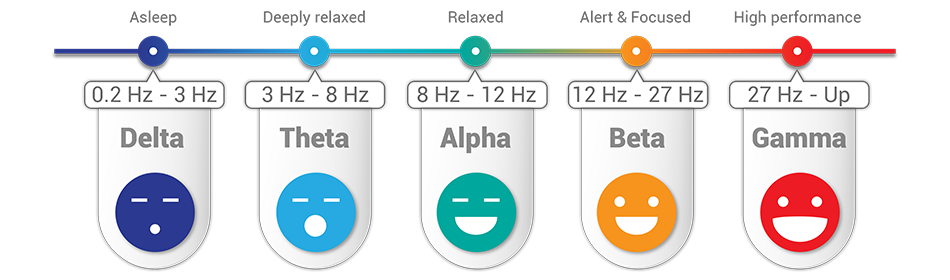
\includegraphics[height=4cm]{brainwavefrequencies.png}
\caption{Brain Wave Classification based on frequency}
\label{fig-1-1}
\end{figure}

\section{Electroencephalography}

Electroencephalography (EEG) is a physiological monitoring method to record electrical activity of the brain. Electroencephalography records the electrical activity of the brain using electrodes placed on the scalp. Measuring electrical activity from the brain is useful because it reflects how the many different neurons in the brain network communicate with each other via electrical impulses.

\subsection{10-20 electrode system}
\begin{figure}[H]
\centering
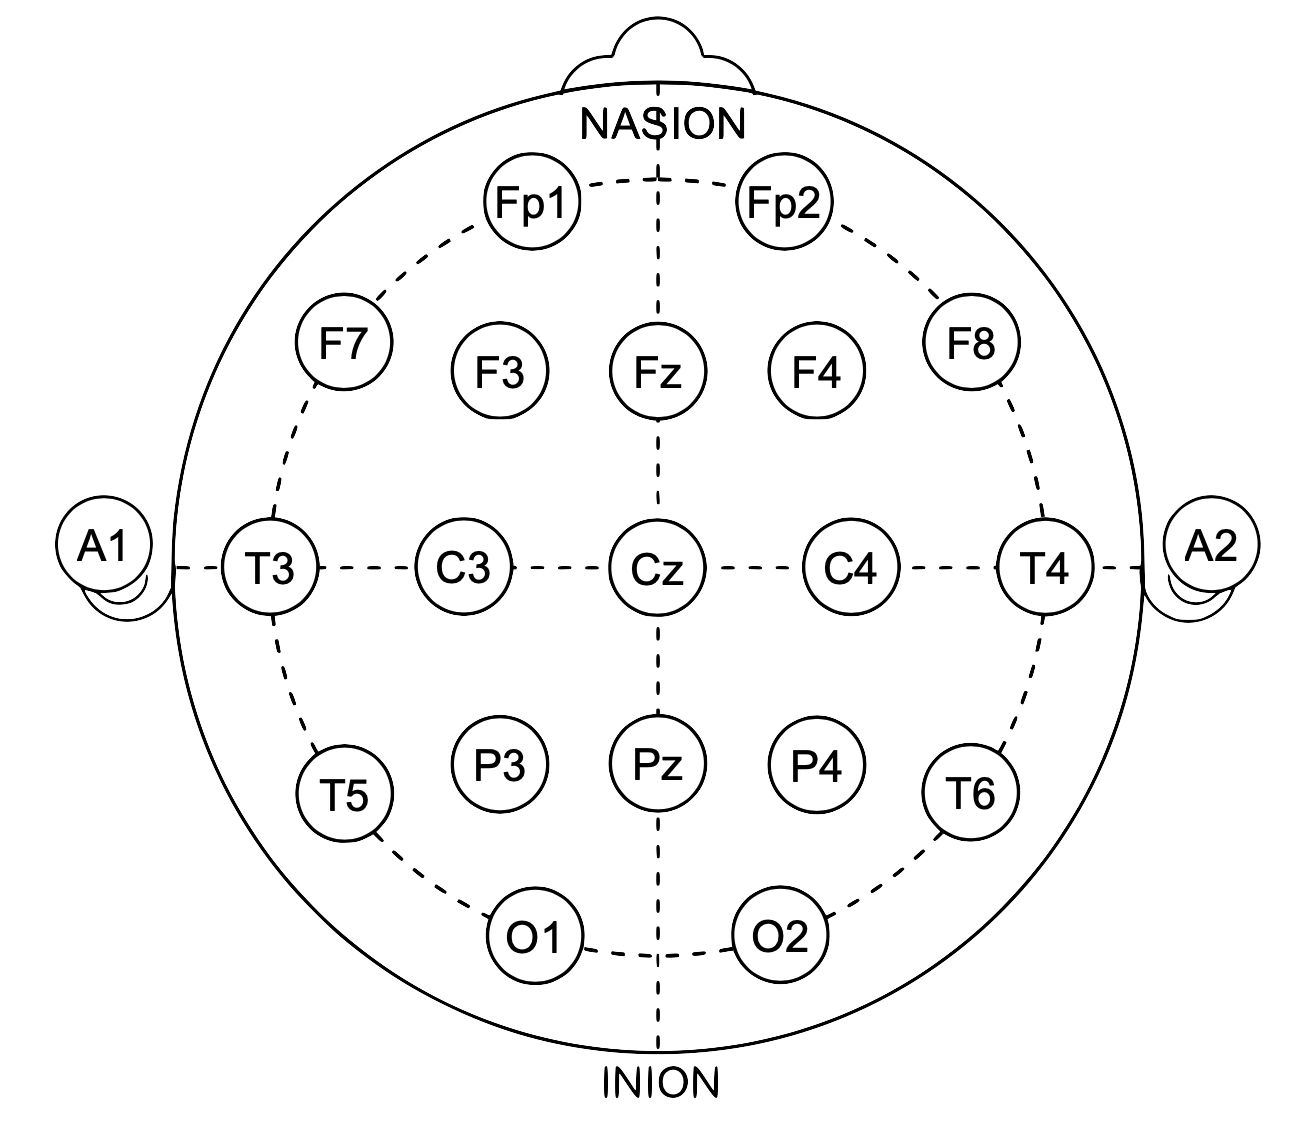
\includegraphics[height=7cm]{1020.png}
\caption{The 10-20 electrode system with 32 electrodes}
\label{fig-1-2}
\end{figure}

In the 10-20 system, electrode names begin with one or two letters indicating the general brain region or lobes where the electrode is placed:

\bfseries \normalfont
\begin{tasks}[label-align=left, label-offset={0mm}, label-width={5mm}, item-indent={5mm}, label-format={\bfseries}, column-sep=10mm](4)
\task \textbf{Fp} Frontopolar
\task \textbf{F} Frontal
\task \textbf{C} Central
\task \textbf{P} Parietal
\task \textbf{O} Occipital
\task \textbf{T} Temporal
\end{tasks}

Each electrode name ends with a number or letter indicating the distance to the midline. Odd numbers are used in the left hemisphere, even numbers in the right hemisphere. Larger numbers indicate greater distances from the midline, while electrodes placed at the midline are labeled with a z for zero. For example, Cz is placed over midline central brain regions, Fp8 is placed over right fronto-polar brain regions, and T7 is placed over left temporal regions.